\subsection{Função Objetivo}
% TODO: add equations, describe variables

Composição da função objetivo:
\begin{itemize}
  \item KICK{\_}POS{\_}VARIATION
  \item WEIGHT{\_}MOVE{\_}DIST{\_}TOTAL
  \item WEIGHT{\_}MOVE{\_}CHANGE
  \item WEIGHT{\_}MOVE{\_}DIST{\_}MAX
  \item TOTAL{\_}MAX{\_}GAP{\_}RATIO
% TOTAL_MAX_GAP_RATIO
% gap_value(){
%   return TOTAL_MAX_GAP_RATIO * total_gap + (1 - TOTAL_MAX_GAP_RATIO) * max_gap;
% }
  \item WEIGHT{\_}ATTACK
  \item WEIGHT{\_}SEE{\_}ENEMY{\_}GOAL
  \item WEIGHT{\_}BLOCK{\_}GOAL
  \item WEIGHT{\_}BLOCK{\_}ATTACKER
  \item WEIGHT{\_}RECEIVERS{\_}NUM
  \item DIST{\_}GOAL{\_}PENAL
  \item DIST{\_}GOAL{\_}TO{\_}PENAL
\end{itemize}

Além dos parâmetros listados acima, outros parâmetros
afetam o comportamento do time:
\begin{itemize}
  \item MIN{\_}GAP{\_}TO{\_}KICK
  \item RAMIFICATION{\_}NUMBER
\end{itemize}

Esses parâmetros serão detalhados a seguir.

KICK{\_}POS{\_}VARIATION: o objetivo deste parâmetro é incorporar a monvimentação
do atacante no cálculo do \textit{gap} do gol. Isso pois defensores mais
próximos são mais facilmente driblados que defensores mais distantes. Isso
pode ser visualizado na figura \ref{fig:kick_pos_1}, onde foi considerada
uma variação de 15cm. Já na figura \ref{fig:kick_pos_2} foi considerada uma
variação de 0cm na posição da bola. Essa variação é medida na linha normal
à reta formada pela bola e pelo robô em questão.

\begin{figure}[h]
  \centering
  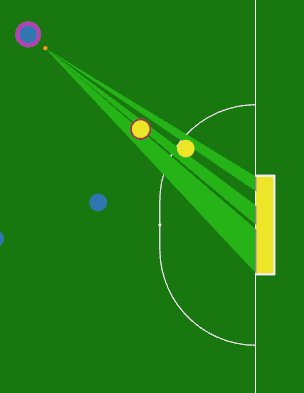
\includegraphics[width=0.8\linewidth]{kick_pos_var_1}
  \caption{\textit{Gap} do gol considerando-se uma variação de 15cm na 
           posição da bola}\label{fig:kick_pos_1}
  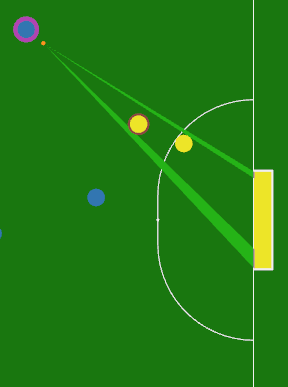
\includegraphics[width=0.8\linewidth]{kick_pos_var_2}
  \caption{\textit{Gap} do gol sem variação de na posição da
           bola}\label{fig:kick_pos_1}
\end{figure}


WEIGHT{\_}MOVE{\_}DIST{\_}TOTAL: o objetivo deste parâmetro é incorporar o custo da
mudança de estado na função objetivo. Ele é formado pela soma dos \textit{
moves} de todos os robôs do time em questão.

WEIGHT{\_}MOVE{\_}DIST{\_}MAX: o objetivo deste parâmetro é incorporar o custo da
mudança de estado na função objetivo. Ele é formado pelo \textit{move}
maior do planejamento atual.

WEIGHT{\_}MOVE{\_}CHANGE: o objetivo deste parâmetro é evitar mudanças grandes no
planejamento do move. Uma das razões para isso é evitar um mode dinâmico
exato neste nível de planejamento, já que isso aumentaria muito o custo
computacional desta etapa do planejamento e, consequentemente, reduziria
o número de simulações possíveis. Por essas razões mudanças no planejamento
dos \textit{moves} são penalizadas de acordo com a distância euclidiana
entre o $move_p$ planejado anteriormente e o $move_mr$} modificado.
Isso permite que sejam selecionados $moves_m$ mais próximos do
$move_p$, refinado assim o planejamento anterior.


TOTAL{\_}MAX{\_}GAP{\_}RATIO: o objetivos deste parâmetro é valorizar \textit{gaps} maiores
de acordo com a soma total dos \textit{gaps} e com o maior \textit{gap}.
O cálculo do \textit{gap} é feito da seguinte maneira:

\begin{dmath} 
 gap value = TOTAL\_MAX\_GAP\_RATIO . \sum gap_i + (1 - TOTAL\_MAX\_GAP\_RATIO) .
 \lbrace maxgap_i \rbrace
\end{dmath} 

WEIGHT{\_}ATTACK
WEIGHT{\_}SEE{\_}ENEMY{\_}GOAL
WEIGHT{\_}BLOCK{\_}GOAL
WEIGHT{\_}BLOCK{\_}ATTACKER
WEIGHT{\_}RECEIVERS{\_}NUM

DIST{\_}GOAL{\_}PENAL
DIST{\_}GOAL{\_}TO{\_}PENAL
